\begin{figure*}[t]
    \centering
    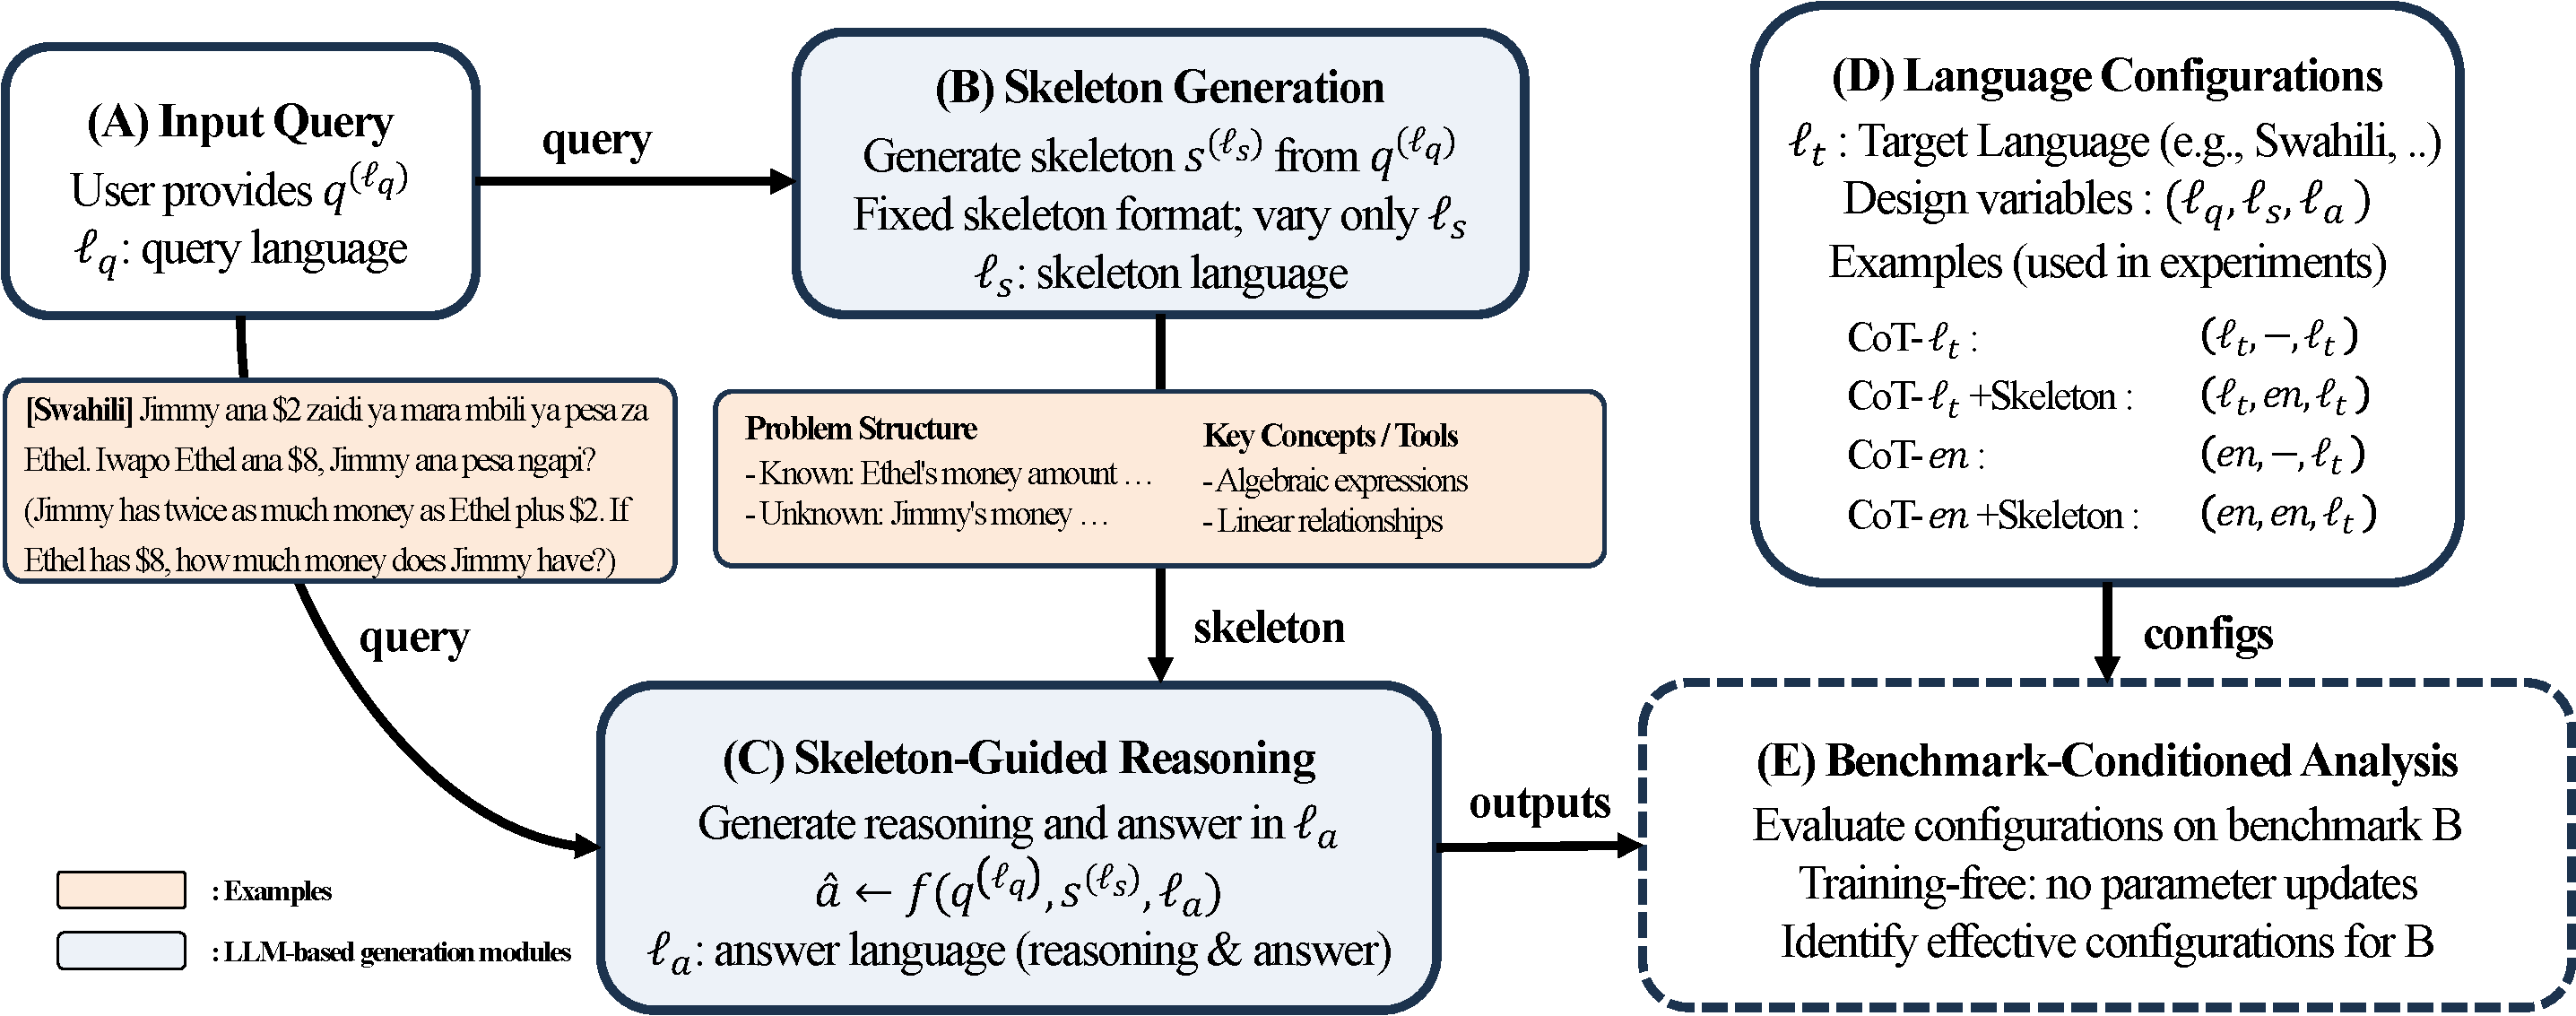
\includegraphics[width=\textwidth]{Figures/Images/LASOF3.pdf}
    \caption{\small Overview of the Skeleton-Guided Reasoning Framework. (A) The process begins with an input query $q^{(\ell_q)}$. (B) A structured skeleton $s^{(\ell_s)}$ is generated to abstract the problem logic. (C) The final reasoning and answer $\hat{a}$ are produced in the answer language $\ell_a$, conditioned on the query and skeleton. (D) We define the language configuration space as $(\ell_q, \ell_s, \ell_a)$ and compare four primary strategies: standard CoT and skeleton-guided approaches, applied in both the target language ($\ell_t$) and English ($en$). (E) Effective configurations are identified through training-free benchmark analysis.
}
\label{fig:figure1}
    \vspace{-0.15in}
\end{figure*}


\section{Language-Aware Skeleton Exploration Framework}

% This study investigates how the effectiveness of skeleton-based reasoning varies depending on language choice and evaluation contexts within a multilingual environment. To this end, we propose the \emph{Language-Aware Skeleton Exploration Framework (\Lasef)}, which systematically analyzes skeleton utilization by varying language configurations while keeping the structure and format of the skeleton fixed. Here, ``exploration'' does not refer to new training or algorithmic search, but rather to an empirical analysis process designed to identify effective language configurations within a given evaluation environment.

This study investigates how the effectiveness of skeleton-based reasoning varies depending on language choice and evaluation contexts within a multilingual environment. To this end, we propose the \emph{Language-Aware Skeleton Exploration Framework (\Lasef)}, as illustrated in Fig.~\ref{fig:figure1}, which systematically analyzes skeleton utilization by varying language configurations while keeping the structure and format of the skeleton fixed. Here, ``exploration'' does not refer to new training or algorithmic search, but rather to an empirical analysis process designed to identify effective language configurations within a given evaluation environment.


\subsection{Problem Setup and Language Dimensions}

Standard language model inference typically involves a query $q$ and a corresponding answer $a$, where the query is presented in a specific language $\ell_q$. In skeleton-based reasoning, the model first generates a skeleton $s$, summarizing the core structure required for problem-solving based on the query, and subsequently uses it to generate the detailed reasoning process and the final answer. This process entails three distinct language choices given a user's target language $\ell_t$: (1) the language of the query, $\ell_q$; (2) the language of the skeleton, $\ell_s$; and (3) the language in which the detailed reasoning and final answer are generated, $\ell_a$.

These three languages may be identical or distinct; depending on their combination, the linguistic priors and reasoning paths elicited by the model can vary. Thus, a single skeleton-based reasoning process is characterized by the language combination $(\ell_q, \ell_s, \ell_a)$. \LASEF focuses on isolating and analyzing the impact of these language configurations on reasoning performance while fixing the skeleton generation method and structure. Under this formulation, the skeleton-based reasoning process can be expressed as:
\[
\hat{a} = f\big(q^{(\ell_q)}, s^{(\ell_s)}, \ell_a\big),
\]

where $f(\cdot)$ represents the inference function of the pre-trained language model, and $s^{(\ell_s)}$ denotes the skeleton expressed in language $\ell_s$.

Notably, the effective language combination for skeleton utilization is not universally fixed but may vary depending on the benchmark or domain used for evaluation. Given a specific benchmark $B$ consisting of query-answer pairs $(\{q,a\} \in B)$, \LASEF provides an analytical framework to identify relatively effective skeleton language configurations within that evaluation environment by comparing performance variations under different language combinations $(\ell_q, \ell_s, \ell_a)$.

This problem setup assumes a \emph{training-free} environment involving no additional training or parameter updates. The following section describes the specific language configurations and skeleton usage methods considered in this study.

\subsection{Skeleton Construction and Usage}

The skeletons used in this study are intermediate representations that concisely reveal the \emph{reasoning structure} for problem-solving, rather than presenting core answers or calculation procedures. In other words, the skeleton provides a minimal structural guide for the reasoning process to follow, avoiding specific instructions for the actual solution steps. This perspective conceptually aligns with existing research interpreting skeletons as structural representations that organize reasoning, rather than as summaries or hints for the solution.

Accordingly, our skeletons maintain a very short and abstract form, excluding specific calculation steps or answers%\footnote{Using longer skeletons risks leaking solution strategies into the prompt, which would confound our goal of isolating the effect of language choice from that of explicit reasoning supervision.}
. To ensure this, we consistently apply the following principle during skeleton generation: \emph{``Provide only the essential structural characteristics of the problem. Describe what the problem structure is, never how to solve it.''}

Fig.~\ref{fig:figure1} presents a representative example of a skeleton generated in English ($\ell_s=en$) for a Swahili query ($\ell_q=sw$). Adhering to our proposed criteria, skeletons maintain a concise length of approximately 120 tokens on average regardless of the language, devoid of direct answers or core solution steps. We provide a detailed quantitative analysis of skeleton length and content distribution, along with the complete generation rules and additional examples, in Appendix~\ref{Appendix:about-skeleton}.